\documentclass[../main.tex]{subfiles}
\begin{document}

\chapter{Finite elements in 2D and 3D}
	\label{chap:chap_9}
	\noindent Finite element approximation is particularly powerful in $2 \mathrm{D}$ and 3D because the method can handle a geometrically complex domain $\Omega$ with ease. The principal idea is, as in $1 \mathrm{D}$, to divide the domain into cells and use polynomials for approximating a function over a cell. Two popular cell shapes are triangles and the quadrilaterals. Figures \hyperref[fig:img_34]{34}, \hyperref[fig:img_35]{35} , and \hyperref[fig:img_36]{36} provide examples. $\mathrm{P} 1$ elements means linear functions $\left(a_{0}+a_{1} x+a_{2} y\right)$ over triangles, while Q1 elements have bilinear functions $\left(a_{0}+a_{1} x+a_{2} y+a_{3} x y\right)$ over rectangular cells. Higher-order elements can easily be defined.
	\begin{figure}[H]
		\centering
		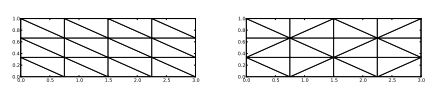
\includegraphics[width=0.7\linewidth]{img_34}
		\caption{Examples on 2D P1 elements.}
		\label{fig:img_34}
	\end{figure}
	\begin{figure}[H]
		\centering
		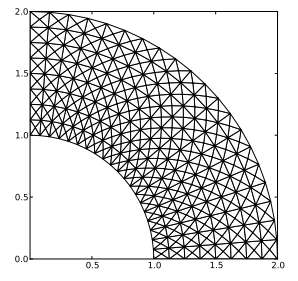
\includegraphics[width=0.7\linewidth]{img_35}
		\caption{Examples on 2D P1 elements in a deformed geometry.}
		\label{fig:img_35}
	\end{figure}
	\section[Basis functions over triangles in the physical domain]{Basis functions over triangles in the physical domain}
	\label{sec:sec_9_1}
	\noindent Cells with triangular shape will be in main focus here. With the $\mathrm{P} 1$ triangular element, $u$ is a linear function over each cell, as depicted in Figure \hyperref[fig:img_37]{37}, with discontinuous derivatives at the cell boundaries.
	
	We give the vertices of the cells global and local numbers as in 1D. The degrees of freedom in the $\mathrm{P} 1$ element are the function values at a set of nodes, which are the three vertices. The basis function $\varphi_{i}(x, y)$ is then 1 at the vertex with global vertex number $i$ and zero at all other vertices. On an element, the three degrees of freedom uniquely determine the linear basis functions in that element, as usual. The global $\varphi_{i}(x, y)$ function is then a combination of the linear functions (planar surfaces) over all the neighboring cells that have vertex number $i$ in common. Figure \hyperref[fig:img_38]{38} tries to illustrate the shape of such a "pyramid"-like function.
	\begin{figure}[H]
		\centering
		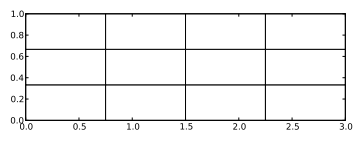
\includegraphics[width=0.7\linewidth]{img_36}
		\caption{Examples on 2D Q1 elements.}
		\label{fig:img_36}
	\end{figure}
	
	\noindent \textbf{Element matrices and vectors}. As in $1 \mathrm{D}$, we split the integral over $\Omega$ into a sum of integrals over cells. Also as in 1D, $\varphi_{i}$ overlaps $\varphi_{j}$ (i.e., $\varphi_{i} \varphi_{j} \neq 0$ ) if and only if $i$ and $j$ are vertices in the same cell. Therefore, the integral of $\varphi_{i} \varphi_{j}$ over an element is nonzero only when $i$ and $j$ run over the vertex numbers in the element. These nonzero contributions to the coefficient matrix are, as in 1D, collected in an element matrix. The size of the element matrix becomes $3 \times 3$ since there are three degrees of freedom that $i$ and $j$ run nver. Again, as in 1D, we number the local vertices in a cell, starting at 0 , and add the entries in the element matrix into the global system matrix, exactly as in 1D. All details and code appear below.
	\bigbreak
	\section[Basis functions over triangles in the reference cell]{Basis functions over triangles in the reference cell}
	\label{sec:sec_9_2}
	\noindent As in 1D, we can define the basis functions and the degrees of freedom in a reference cell and then use a mapping from the reference coordinate system to the physical coordinate system. We also have a mapping of local degrees of freedom numbers to global degrees of freedom numbers.
	
	The reference cell in an $(X, Y)$ coordinate system has vertices $(0,0),(1,0)$, and $(0,1)$, corresponding to local vertex numbers 0,1 , and 2 , respectively. The $\mathrm{P} 1$ element has linear functions $\tilde{\varphi}_{r}(X, Y)$ as basis functions, $r=0,1,2$. Since a linear function $\tilde{\varphi}_{r}(X, Y)$ in $2 \mathrm{D}$ is on the form $C_{r, 0}+C_{r, 1} X+C_{r, 2} Y$, and hence has three parameters $C_{r, 0}, C_{r, 1}$, and $C_{r, 2}$, we need three degrees of freedom. These are in general taken as the function values at a set of nodes. For the P1
	\begin{figure}[H]
		\centering
		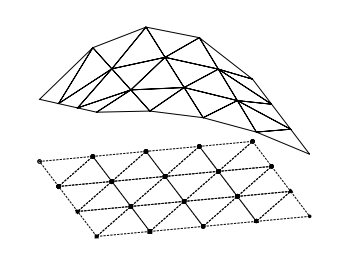
\includegraphics[width=0.7\linewidth]{img_37}
		\caption{Example on piecewise linear 2D functions defined on triangles.}
		\label{fig:img_37}
	\end{figure}
	\noindent element the set of nodes is the three vertices. Figure \hyperref[fig:img_39]{39} displays the geometry of the element and the location of the nodes.
	
	Requiring $\tilde{\varphi}_{r}=1$ at node number $r$ and $\tilde{\varphi}_{r}=0$ at the two other nodes, gives three linear equations to determine $C_{r, 0}, C_{r, 1}$, and $C_{r, 2}$. The result is
	\begin{equation}\label{eqa109}
		\tilde{\varphi}_{0}(X, Y)=1-X-Y,
	\end{equation}
	\begin{equation}\label{eqa110}
		\tilde{\varphi}_{1}(X, Y)=X,
	\end{equation}
	\begin{equation}\label{eqa111}
		\tilde{\varphi}_{2}(X, Y)=Y
	\end{equation}
	Higher-order approximations are obtained by increasing the polynomial order, adding additional nodes, and letting the degrees of freedom be function values at the nodes. Figure \hyperref[fig:img_40]{40} shows the location of the six nodes in the P2 element.
	A polynomial of degree $p$ in $X$ and $Y$ has $n_{p}=(p+1)(p+2) / 2$ terms and hence needs $n_{p}$ nodes. The values at the nodes constitute $n_{p}$ degrees of freedom. The location of the nodes for $\tilde{\varphi}_{r}$ up to degree 6 is displayed in Figure \hyperref[fig:img_41]{41}.
	
	The generalization to $3 \mathrm{D}$ is straightforward: the reference element is a \href{https://en.wikipedia.org/wiki/Tetrahedron}{tetrahedron} with vertices $(0,0,0),(1,0,0),(0,1,0)$, and $(0,0,1)$ in a $X, Y, Z$ reference coordinate system. The $\mathrm{P} 1$ element has its degrees of freedom as four nodes, which are the four vertices, see Figure \hyperref[fig:img_42]{42} . The $\mathrm{P} 2$ element adds additional nodes along the edges of the cell, yielding a total of 10 nodes and degrees of freedom, see Figure \hyperref[fig:img_43]{43} .
	
	The interval in 1D, the triangle in 2D, the tetrahedron in 3D, and its generalizations to higher space dimensions are known as \textit{simplex} cells (the
	\begin{figure}[H]
		\centering
		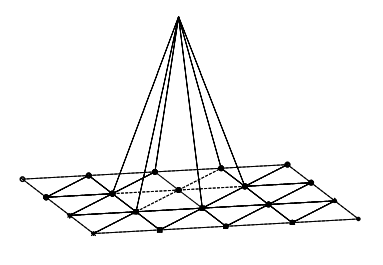
\includegraphics[width=0.7\linewidth]{img_38}
		\caption{Example on a piecewise linear 2D basis function over a patch of
			triangles.}
		\label{fig:img_38}
	\end{figure}
	\begin{figure}[H]
		\centering
		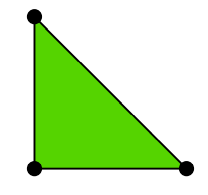
\includegraphics[width=0.7\linewidth]{img_39}
		\caption{2D P1 element.}
		\label{fig:img_39}
	\end{figure}
	
	\noindent geometry) or \textit{simplex} elements (the geometry, basis functions, degrees of freedom,
	etc.). The plural forms \href{https://en.wikipedia.org/wiki/Simplex}{simplices} and simplexes are also a much used shorter
	terms when referring to this type of cells or elements. The side of a simplex is
	called a \textit{face}, while the tetrahedron also has \textit{edges}.
	
	Acknowledgment. Figures \hyperref[fig:img_39]{39} to \hyperref[fig:img_43]{43} are created by Anders Logg and taken
	from the \href{https://launchpad.net/fenics-book}{FEniCS book}: \textit{Automated Solution of Differential Equations by the
		Finite Element Method}, edited by A. Logg, K.-A. Mardal, and G. N. Wells,
	published by \href{https://link.springer.com/book/10.1007/978-3-642-23099-8}{Springer}, 2012.
	\begin{figure}[H]
		\centering
		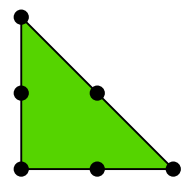
\includegraphics[width=0.7\linewidth]{img_40}
		\caption{2D P2 element.}
		\label{fig:img_40}
	\end{figure}
	\begin{figure}[H]
		\centering
		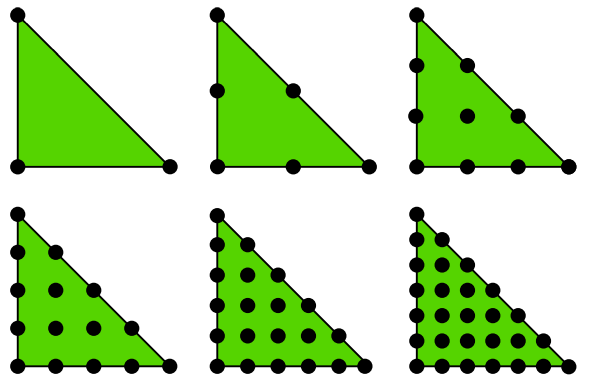
\includegraphics[width=0.7\linewidth]{img_41}
		\caption{2D P1, P2, P3, P4, P5, and P6 elements.}
		\label{fig:img_41}
	\end{figure}
	\section[Affine mapping of the reference cell]{Affine mapping of the reference cell}
	\label{sec:sec_9_3}
	\noindent Let $\tilde{\varphi}_{r}^{(1)}$ denote the basis functions associated with the $\mathrm{P} 1$ element in $1 \mathrm{D}, 2 \mathrm{D}$, or 3D, and let $\boldsymbol{x}_{q(e, r)}$ be the physical coordinates of local vertex number $r$ in cell $e$. Furthermore, let $\boldsymbol{X}$ be a point in the reference coordinate system corresponding to the point $\boldsymbol{x}$ in the physical coordinate system. The affine mapping of any $\boldsymbol{X}$ onto $\boldsymbol{x}$ is then defined by
	\begin{equation}\label{eqa112}
		x=\sum_{r} \tilde{\varphi}_{r}^{(1)}(X) x_{q(e, r)},
	\end{equation}
	where $r$ runs over the local vertex numbers in the cell. The affine mapping essentially stretches, translates, and rotates the triangle. Straight or planar
	\begin{figure}[H]
		\centering
		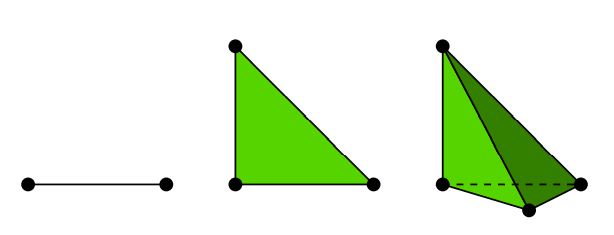
\includegraphics[width=0.7\linewidth]{img_42}
		\caption{P1 elements in 1D, 2D, and 3D.}
		\label{fig:img_42}
	\end{figure}
	\begin{figure}[H]
		\centering
		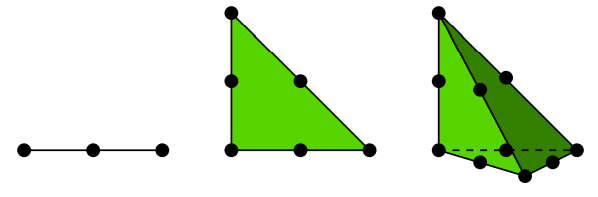
\includegraphics[width=0.7\linewidth]{img_43}
		\caption{P2 elements in 1D, 2D, and 3D.}
		\label{fig:img_43}
	\end{figure}
	
	\noindent faces of the reference cell are therefore mapped onto straight or planar faces
	in the physical coordinate system. The mapping can be used for both P1 and
	higher-order elements, but note that the mapping itself always applies the P1
	basis functions.
	\section[Isoparametric mapping of the reference cell]{Isoparametric mapping of the reference cell}
	\label{sec:sec_9_4}
	Instead of using the $\mathrm{P} 1$ basis functions in the mapping (\hyperref[eqa112]{112}), we may use the basis functions of the actual $\mathrm{Pd}$ element:
	\begin{equation}\label{eqa113}
		x=\sum_{r} \tilde{\varphi}_{r}(X) x_{q(e, r)},
	\end{equation}
	where $r$ runs over all nodes, i.e., all points associated with the degrees of freedom. This is called an \textit{isoparametric mapping}. For P1 elements it is identical to the affine mapping (\hyperref[eqa112]{112}), but for higher-order elements the mapping of the straight or planar faces of the reference cell will result in a \textit{curved} face in the physical coordinate system. For example, when we use the basis functions of the triangular P2 element in $2 \mathrm{D}$ in (\hyperref[eqa113]{113}), the straight faces of the reference triangle are mapped onto curved faces of parabolic shape in the physical coordinate system, see Figure \hyperref[fig:img_45]{45} .
	\begin{figure}[H]
		\centering
		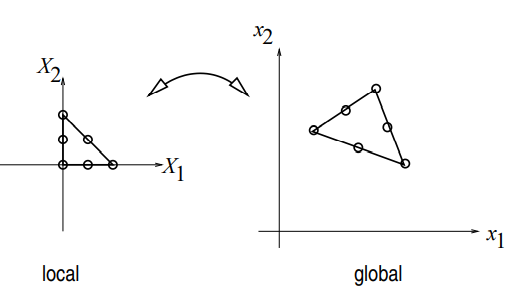
\includegraphics[width=0.7\linewidth]{img_44}
		\caption{Affine mapping of a P1 element.}
		\label{fig:img_44}
	\end{figure}
	\begin{figure}[H]
		\centering
		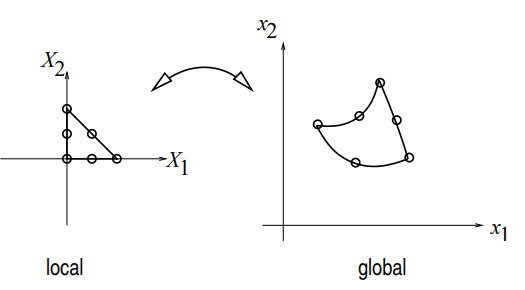
\includegraphics[width=0.7\linewidth]{img_45}
		\caption{Isoparametric mapping of a P2 element.}
		\label{fig:img_45}
	\end{figure}
	
	From (\hyperref[eqa112]{112}) or (\hyperref[eqa113]{113}) it is easy to realize that the vertices are correctly mapped. Consider a vertex with local number $s$. Then $\tilde{\varphi}_{s}=1$ at this vertex and zero at the others. This means that only one term in the sum is nonzero and $\boldsymbol{x}=\boldsymbol{x}_{q(e, s)}$, which is the coordinate of this vertex in the global coordinate system.
	\section[Computing integrals]{Computing integrals}
	\label{sec:sec_9_5}
	Let $\tilde{\Omega}^{r}$ denote the reference cell and $\Omega^{(e)}$ the cell in the physical coordinate system. The transformation of the integral from the physical to the reference coordinate system reads
	\begin{equation}\label{eqa114}
		\int_{\Omega^{(e)}} \varphi_{i}(\boldsymbol{x}) \varphi_{j}(\boldsymbol{x}) \mathrm{d} x =\int_{\tilde{\Omega}^{r}} \tilde{\varphi}_{i}(\boldsymbol{X}) \tilde{\varphi}_{j}(\boldsymbol{X}) \operatorname{det} J \mathrm{~d} X
	\end{equation}
	\begin{equation}\label{eqa115}
		\int_{\Omega^{(e)}} \varphi_{i}(\boldsymbol{x}) f(\boldsymbol{x}) \mathrm{d} x =\int_{\tilde{\Omega}^{r}} \tilde{\varphi}_{i}(\boldsymbol{X}) f(\boldsymbol{x}(\boldsymbol{X})) \operatorname{det} J \mathrm{~d} X
	\end{equation}
	
	\noindent where $\mathrm{d} x$ means the infinitesimal area element $d x d y$ in $2 \mathrm{D}$ and $d x d y d z$ in 3D, with a similar definition of $\mathrm{d} X$. The quantity det $J$ is the determinant of the Jacobian of the mapping $\boldsymbol{x}(\boldsymbol{X})$. In 2D,
	\begin{equation}\label{eqa116}
		J=\left[\begin{array}{ll}
			\frac{\partial x}{\partial X} & \frac{\partial x}{\partial Y} \\
			\frac{\partial y}{\partial X} & \frac{\partial y}{\partial Y}
		\end{array}\right], \quad \operatorname{det} J=\frac{\partial x}{\partial X} \frac{\partial y}{\partial Y}-\frac{\partial x}{\partial Y} \frac{\partial y}{\partial X} .
	\end{equation}
	With the affine mapping (\hyperref[eqa112]{112}), $\operatorname{det} J=2 \Delta$, where $\Delta$ is the area or volume of the cell in the physical coordinate system.
	\bigbreak
	\noindent \textbf{Remark.} Observe that finite elements in 2D and 3D builds on the same ideas and \textit{concepts} as in $1 \mathrm{D}$, but there is simply much more to compute because the specific mathematical formulas in 2D and $3 \mathrm{D}$ are more complicated and the book keeping with dof maps also gets more complicated. The manual work is tedious, lengthy, and error-prone so automation by the computer is a must.
\clearpage
\end{document} 
